\title{Evaluation of Supervised Learning Models}
\label{chp:evaluation-supervised-learning}
\author{George G. Cabral and Leandro L. Minku}
\institute{G. Cabral is with the Department of Computing, Federal Rural University
of Pernambuco, BR. L. Minku is with the School of Computer Science, University of Birmingham, UK.}
\maketitle


As explained in the introduction to Part III of this book, supervised learning aims at creating functions (models) able to predict output variables given the values of the input variables. Such functions should be able to generalize to new examples that are unseen at training time. If a predictive model works well on the training data, this does not mean that it works well for unseen data. But how to evaluate how well a given predictive model is likely to perform on unseen data? This chapter will explain a number of performance metrics (Section \ref{sec:supervised-evaluation-metrics}) and evaluation procedures (Section \ref{sec:supervised-evaluation-procedures}) that can be used for this purpose. 


\section{Evaluation Metrics}
\label{sec:supervised-evaluation-metrics}

This section explains some evaluation metrics that can be computed over a set of examples to show how well a given predictive model performs on this set of examples. In other words, they can be used to compute the predictive performance of a given model on a set of examples. Section \ref{sec:eval-metrics-classification} presents evaluation metrics for classification problems, whose output variables are categories. Section \ref{sec:eval-metrics-regression} presents evaluation metrics for regression problems, whose output variables are numeric.

\subsection{Classification Problems}
\label{sec:eval-metrics-classification}

Consider a set of examples with known output values 

\[\mathcal{E} = \{(\mathbf{x}^{(1)},y^{(1)}), (\mathbf{x}^{(2)},y^{(2)}), \cdots, (\mathbf{x}^{(M)},y^{(M)})\},\] 

\noindent where $\mathbf{x}^{(i)} \in \mathcal{X}$ are the input variables coming from any input domain $\mathcal{X}$, $y^{(i)} \in \mathcal{Y}$ is the output variable coming from the categorical domain $\mathcal{Y}$, $1 \leq i \leq M$, and $M$ is the number of examples.  Consider also the predictions $\{\hat{y}^{(1)},\hat{y}^{(2)}, \cdots, \hat{y}^{(M)}\}$ given by a function $f: \mathcal{X} \rightarrow \mathcal{Y}$ to these examples. Each prediction $\hat{y}^{(i)}$ can be either correct or incorrect. It is correct when $\hat{y}^{(i)} = y^{(i)}$ and incorrect when $\hat{y}^{(i)} \neq y^{(i)}$.

When we are dealing with binary classification problems (i.e., problems where $\mathcal{Y}$ is a set containing two categories), it is common to refer to one of the categories as the ``positive'' category and the other one as the ``negative'' category. A matrix called \textit{confusion matrix} can be used to count the number of positive and negative examples from $\mathcal{E}$ that are correctly and incorrectly classified by the function $f$ being evaluated as follows:

\begin{center}
Confusion Matrix:
\begin{tabular}{|c|c|c|}\hline
     & Predicted Positive & Predicted Negative \\ \hline
Actual Positive     &   True Positive (TP)    &   False Negative (FN)    \\ \hline
Actual Negative     &   False Positive (FP)   &   True Negative (TN)    \\ \hline
\end{tabular}
\end{center}

The true positive (TP) is the number of examples that are predicted as positive and are actually positive. The false positive (FP) is the number of examples that are predicted as negative but are actually positive. The True Negative (TN) is the number of examples that are predicted as negative and are actually negative. The False Negative (FN) is the number of examples that are predicted as negative but are actually positive.

The confusion matrix can give an idea of how well the function $f$ is predicting examples in $\mathcal{E}$. However, it is typically easier to interpret the predictive performance of a function when we represent the values above in the form of ratios, or when we aggregate these values into single metric values. We explain below some examples of evaluation metrics that can be computed based on the confusion matrix. 


\textbf{Accuracy} is the proportion of examples that are correctly classified. It can be calculated as follows:

\[ \text{Accuracy} = \frac{TP + TN}{TP+FP+TN+FN}. \]

\noindent This metric has values in $[0,1]$, with 0 being the worst possible value and 1 being the best possible value. 
However, this metric is only suitable when the number of positive and negative examples in $\mathcal{E}$ is similar. When that is not the case (i.e., when the data are \textit{class imbalanced}), this metric focuses on the predictions given for examples of the majority class. Therefore, a function $f$ that is able to predict the majority class very well, but fails to correctly identify examples of the minority class, gets a misleadingly high value for the accuracy metric. For example, consider a problem where $\mathcal{E}$ contains 100 examples -- 10 belonging to the positive class and 90 belonging to the negative class. Consider that $f$ always predicts negative, no matter the values of the input variables of the examples. The accuracy of $f$ would be $(90+0)/100 = 90\%$, which appears to be a very good value. However, $f$ is not a reasonable predictive model, as it always predicts the same category regardless of the example being predicted. 

\textbf{Classification Error} is the opposite of Accuracy:

\[\text{Classification Error} = 1 - \text{Accuracy}.\]

\noindent This metric has values in $[0,1]$, with 1 being the worst possible value and 0 being the best possible value.

\textbf{Precision} is the proportion of positive predictions that are correct predictions. It can be calculated as follows:

\[\text{Precision} = \frac{TP}{TP+FP}. \]

\noindent This metric has values in $[0,1]$, with 0 being the worst possible value and 1 being the best possible value. This metric has also been discouraged for class imbalanced problems, as it is a biased metric \cite{LuqueEtAl2019}.

\textbf{Recall (a.k.a., True Positive Rate (TPR) or Sensitivity)} is the proportion of positive examples that are successfully predicted as positive. It can be calculated as follows:

\[TPR = \frac{TP}{TP+FN} = 1 - FNR, \]

\noindent where $FNR$ is the False Negative Rate:

\[FNR = \frac{FN}{TP+FN}. \]

\noindent Recall has values in $[0,1]$, with 0 being the worst possible value and 1 being the best possible value, whereas FNR has values in $[0,1]$, with 1 being the worst possible value and 0 being the best possible value. Recall and FNR are suitable metrics to be used no matter if the data are class imbalanced or not. However, they only represent how well $f$ performs on the positive category. Therefore, they should never be reported in isolation. Other metrics to also capture performance on the negative category, such as the specificity explained below, should be reported to complement them.

\textbf{Specificity (a.k.a., True Negative Rate)}  is the proportion of negative examples that is successfully predicted as negative.  It can be calculated as follows:

\[TNR = \frac{TN}{TN+FP} = 1 - FPR, \]

\noindent where $FPR$ is the False Positive Rate (a.k.a., false alarm rate):

\[FPR = \frac{FP}{TN+FP}. \]

\noindent Specificity has values in $[0,1]$, with 0 being the worst possible value and 1 being the best possible value, whereas FPR has values in $[0,1]$, with 1 being the worst possible value and 0 being the best possible value. Similar to recall and FNR, Specificity and FPR are suitable metrics to be used no matter if the data are class imbalanced or not, but should be complemented by the report of other metrics to also capture performance on the positive category. 

\textbf{F1-Score} is the harmonic mean between precision and recall:

\[ \text{F1-Score} = 2 \cdot \frac{\text{Precision} \cdot \text{Recall}}{\text{Precision} + \text{Recall}}. \]

\noindent It has values in  $[0,1]$, with 0 being the worst possible value and 1 being the best possible value. F1-Score is a useful metric when one needs to aggregate precision and recall into a single value. However, similar to Precision, F1-Score is also a biased metric that has been discouraged for class imbalanced data \cite{LuqueEtAl2019}.

\textbf{G-Mean} is the geometric mean between recall and specificity:

\[\text{G-Mean} = \sqrt{TPR \cdot TNR}.\]

\noindent It has values in  $[0,1]$, with 0 being the worst possible value and 1 being the best possible value.  Similar to Recall and Specificity, G-Mean is suitable for both class balanced and imbalanced data. It is a useful metric when one needs to aggregate the performance on the positive and negative categories into a single unbiased metric.



When dealing with multi-class classification problems (i.e., problems where $\mathcal{Y}$ is a set containing more than two categories), the confusion matrix can be generalized as follows, where $c_i$, represents a given category in $\mathcal{Y}$, $i \in \{1,2,\cdots, n\}$, $n$ is the number of categories, and $C_{j,k}$ is the number of examples of category $c_j$ that were predicted by $f$ as being of category $c_k$, $\forall j,k \in \mathcal{Y}$:

\begin{center}
\begin{tabular}{|c|c|c|c|c|}\hline
     & Predicted $c_1$ & Predicted $c_2$ & $\cdots$ & Predicted $c_n$ \\ \hline
Actual $c_1$     &   $C_{1,1}$   & $C_{1,2}$ & $\cdots$ & $C_{1,n}$       \\ \hline
Actual $c_2$     &   $C_{2,1}$   &  $C_{2,2}$ & $\cdots$ & $C_{2,n}$       \\ \hline
$\vdots$ & \multicolumn{2}{c|}{$\ddots$} & $\cdots$ & $\vdots$ \\ \hline
Actual $c_n$     &   $C_{n,1}$   & $C_{n,2}$ & $\cdots$ &  $C_{n,n}$      \\ \hline
\end{tabular}
\end{center}

Metrics for binary classification problems can also be generalized to multi-class problems. 

The following correspond to the overall accuracy, and to the precision, recall and specificity for a given category $c_i$:

\[ \text{Accuracy} = \frac{\sum_{i=1}^n C_{i,i}}{\sum_{j,k=1}^n C_{j,k}}, \]

\[ \text{Precision}_{c_i} = \frac{C_{i,i}}{\sum_{j=1}^n C_{j,i}}, \]

\[ \text{Recall}_{c_i} = \frac{C_{i,i}}{\sum_{j=1}^n C_{i,j}}, \]

\[ \text{Specificity}_{c_i} = \frac{\sum_{j\neq i} C_{j,j}}{\sum_{j\neq i, k} C_{j,k}}. \]

Based on these, the F1-Score for a given category $c_i$ and the overall G-Mean for all categories can be computed as follows:

\[ \text{F1-Score}_{c_i} = 2 \cdot \frac{ \text{Precision}_{c_i} \cdot \text{Recall}_{c_i}}{\text{Precision}_{c_i} + \text{Recall}_{c_i}}, \]

\[ \text{G-Mean} = \sqrt[n]{\prod_{i=1}^n C_{i,i}}.\]

%AUC may be too advanced for now

\subsection{Regression Problems}
\label{sec:eval-metrics-regression}

Consider a set of examples with known output values 

\[\mathcal{E} = \{(\mathbf{x}^{(1)},y^{(1)}), (\mathbf{x}^{(2)},y^{(2)}), \cdots, (\mathbf{x}^{(M)},y^{(M)})\},\] 

\noindent where $\mathbf{x}^{(i)} \in \mathcal{X}$ are the input variables coming from any input domain $\mathcal{X}$, $y^{(i)} \in \mathcal{R}$ is a real-valued output variable, $1 \leq i \leq M$, and $M$ is the number of examples.  Consider also the predictions $\{y'^{(1)},y'^{(2)}, \cdots, y'^{(M)}\}$ given by a function $f: \mathcal{X} \rightarrow \mathcal{R}$ to these examples. Different from classification problems, instead of considering predictions as ``correct'' or ``incorrect'', it is common practice to check how different the predicted value is from the actual one, i.e., how large the error of the predictions is.  We show below some evaluation metrics that can be used to evaluate $f$ based on $\mathcal{E}$. 

\textbf{Mean Absolute Error (MAE)} is the average absolute value of the difference between the predicted and actual outputs:

\[ MAE = \frac{1}{M} \sum_{i=1}^M |y^{(i)} - \hat{y}^{(i)}|.\]

\noindent This metric has positive or zero values, where the smaller the value the better. 

\textbf{Mean Squared Error (MSE)} is the average squared value of the difference between the predicted and actual outputs:

\[ MSE = \frac{1}{M} \sum_{i=1}^M (y^{(i)} - \hat{y}^{(i)})^2.\]

\noindent This metric has positive or zero values, where the smaller the value the better. The squared function has the effect of emphasizing larger differences between the actual and predicted output values. However, the use of the squared function makes the values of this metric more difficult to interpret, as their unit of measurement is different from the unit of the output variable. The metric presented next overcomes this problem.

\textbf{Root Mean Squared Error (RMSE)} is the squared root of the MSE:

\[ RMSE = \sqrt{\frac{1}{M} \sum_{i=1}^M (y^{(i)} - \hat{y}^{(i)})^2}.\]

\noindent This metric has positive or zero values, where the smaller the value the better. 

The metrics above are measured in the unit of the output variable (or the square unit, in the case of MSE), which may not be very easy to interpret depending on the problem. The metrics explained below may be helpful to improve interpretability. 

\textbf{Mean Absolute Percentage Error (MAPE)} is the absolute value of the difference between the actual and predicted output values as a proportion of the actual value:

\[ MAPE = \frac{1}{M} \sum_{i=1}^M \left|\frac{y^{(i)} - \hat{y}^{(i)}}{y^{(i)}}\right|. \]

\noindent This metric has positive or zero values. Values smaller/larger than one correspond to prediction errors that are in general smaller/larger than the actual output values. The smallest the value of this metric, the better. However, this metric may place less emphasis on errors performed on examples whose output values are larger. This is because larger output values will result in a larger denominator, and as a result a smaller relative error.   

\textbf{Relative Absolute Error (RAE)} is a measure of the error relative to a simple model that would predict the average of the actual output values of the examples in $\mathcal{E}$:

\[RAE = \frac{\sum_{i=1}^M |y^{(i)} - \hat{y}^{(i)}|} {\sum_{i=1}^M |y^{(i)} - \bar{y}|}, \]

\noindent where $\bar{y}$ is the average of the actual outputs:

\[\bar{y} = \frac{1}{M}\sum_{i=1}^M y^{(i)}.\]

\noindent This metric has values that are positive or zero. RAE's numerator represents the MAE of the function $f$ being evaluated, whereas RAE's denominator represents the MAE of the simple model. Therefore, values smaller/larger than 1 mean that the predictions are in general better/worse than those provided by the simple model.

\textbf{Root Relative Squared Error (RRSE)} is also a measure of the error relative to a simple model that would predict $\bar{y}$. However, similar to RMSE, it further emphasizes larger errors by squaring the differences between the actual and predicted output values:

\[RRSE = \sqrt{\frac{\sum_{i=1}^M (y^{(i)} - \hat{y}^{(i)})^2} {\sum_{i=1}^M (y^{(i)} - \bar{y})^2}}. \]

\noindent This metric also has values that are positive or zero, where smaller values are better values. Values that are smaller/larger than 1 mean that the predictions are in general better/worse than those provided by the simple model.

\section{Evaluation Procedures}
\label{sec:supervised-evaluation-procedures}

%The evaluation metrics are part of the tools necessary to assess the quality of a classifier for solving a specific problem. Nevertheless, they do not take into account the arrangement of the data in the hyperspace used to obtain the predictive performance result. 

During the modeling phase of a problem, i.e., when training the predictive model, practitioners have access to a limited amount of training data (i.e., a subset of examples of the problem) and the aim is to create a predictive model that behaves well when deployed (i.e., that can generalize well to unseen data). %Therefore, it is important to extract as much information as possible from the data in such a way that the predictive model generalizes the learned task to unseen cases. 
In an unreal scenario, practitioners would have all possible data available during the modeling (training) phase. In such unreal scenario, theoretically, one could learn a classifier able to produce the best achievable predictive performance (e.g., accuracy of 100\% or MSE of 0). However, in real world problems, the data shortage for modeling the problem is often an issue that must be seriously taken into account. Moreover, data typically includes noisy examples, whose input or output values have been potentially collected with some mistakes. Learning algorithms should try to make the most of the available data while avoiding the negative effect of noise.

%In the worst case, one can manipulate the data in order to obtain a desired result. On the other hand, in order to obtain results as close as possible from the 

Figure \ref{fig:ds1} presents a bi-dimensional two-class dataset where each of the classes contains 20 examples to illustrate this. Assume that these data are used as the training set to learn a classifier. By taking a visual analysis of this dataset we can see some particularities that, intuitively, would be beneficial if incorporated or not incorporated into the classifier:   

\begin{itemize}
    \item Example 20 of the orange class may be interpreted as a noise. It may be desirable for the classifier not to incorporate it into its learned function.
    \item Examples 14, 8 and 15 of the orange class are placed in a conflict area. It may be desirable for the classifier to be capable of separating these examples from those of the blue class. %; and
    %\item Examples far from conflict areas, such as (blue class: 8, 15, 3 and 4) and (orange class: 1, 17, 4 and 7) may not be important for building the classifier, since they aren't placed in the frontier between the classes, but they must not be misclassified. 
\end{itemize}


\begin{figure}[h]
    \centering
    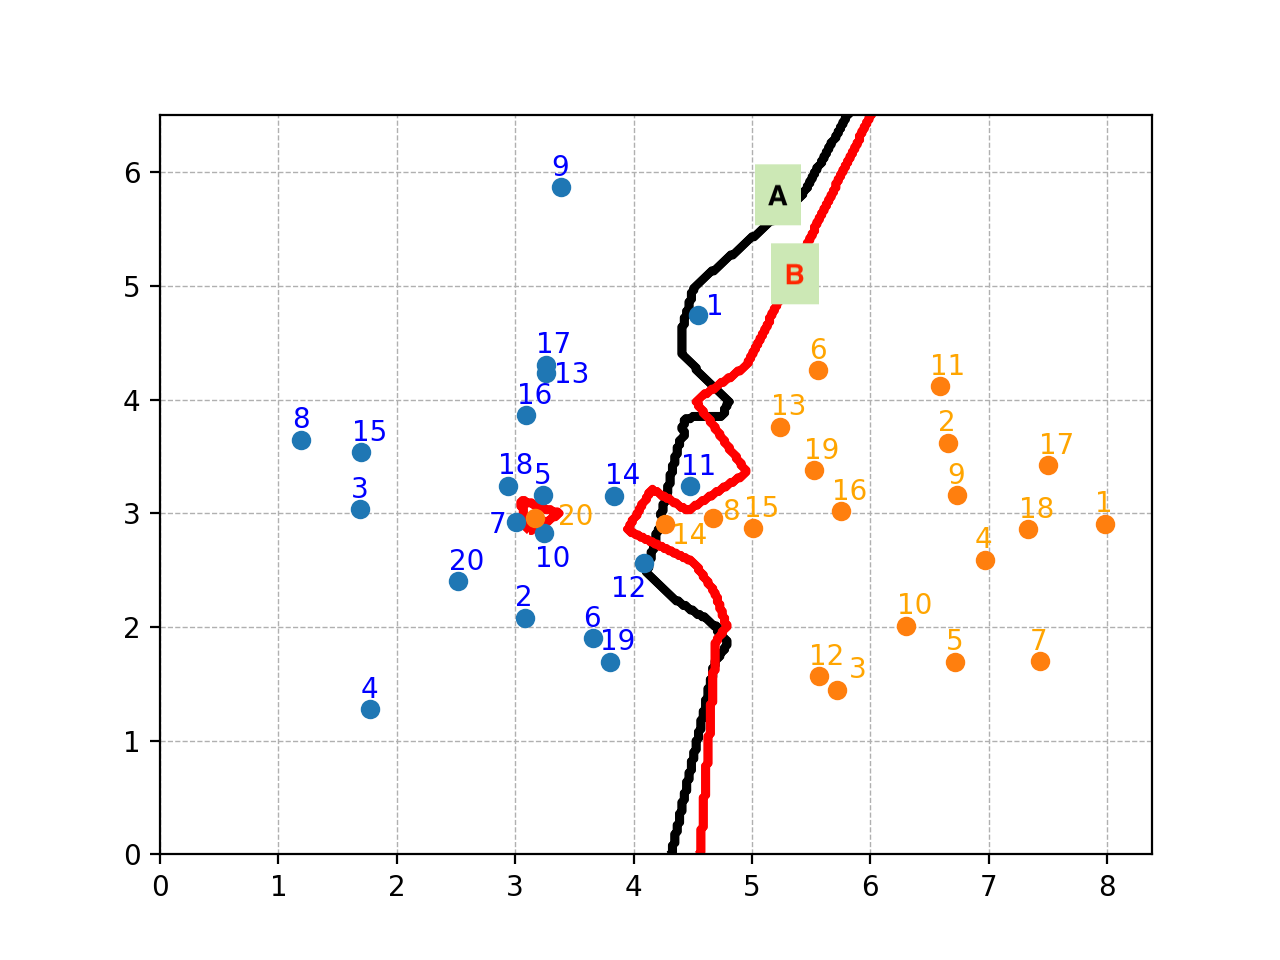
\includegraphics[width=0.9\textwidth]{"Part 3 - Learning Systems/Supervised Learning/Evaluation/Evaluation Supervised/figures/dataset1.png"}
    \caption{Hypothetical 2-class dataset containing 20 examples for each class.}
    \label{fig:ds1}
\end{figure}


As this is a two dimensional problem (with only two input variables), one could attempt to plot the decision boundary learned by the predictive model to get an idea of how well it may generalize to unseen data. The decision boundary are lines learned by a predictive model to separate examples of different classes in a classification problem. As we can see from Figure \ref{fig:ds1}, classifier A was able to make the most of the data while preventing the negative effect of example 20. This classifier is likely to generalize well. However, classifier B learned the noise of example 20. This classifier may not generalize well. Similarly, predictive models for regression problems can also be affected by noise.

In contrast to the dataset presented in Figure \ref{fig:ds1}, most real world problems are composed of several input variables. For these problems we cannot visually assess how good the learned model is.  Instead, we need to compute the predictive performance based on a set of examples using evaluation metrics such as the ones presented in Section \ref{sec:supervised-evaluation-metrics}. However, if we compute the evaluation metrics on the training set, we would be considering a predictive model to be good when it learns noise. For instance, classifier B makes no mistakes on any training example and would get the best possible predictive performance on the training set. In contrast, classifier A misclassifies example 20 and would get worse predictive performance on the training set. Nevertheless, classifier A should be considered as better than classifier B in terms of its generalization capability. 

Evaluation procedures can be used to train predictive models and evaluate their generalization capabilities by splitting the available data into different sets for training and evaluation (testing) purposes. Different evaluation procedures create such splits in different ways. Sections \ref{sec:cv}, \ref{sec:loocv} and \ref{sec:holdout} present three popular evaluation procedures.


\subsection{Stratified $k$-fold Cross-Validation}
\label{sec:cv}

As explained above, when building a classifier, it is imperative that the data used to train the classifier is not used to assess its performance. If a classifier learns a supervised problem represented by a training set $\mathcal{\tau} = \{(\mathbf{x}^{(1)}, y^{(1)}), (\mathbf{x}^{(2)}, y^{(2)}), \cdots, (\mathbf{x}^{(M)}, y^{(M)})$, examples contained in $\mathcal{\tau}$ may be well learned, but examples not present in $\mathcal{\tau}$ may still be misclassified. Therefore, it is important to separate the available data into distinct datasets called training and test datasets. The idea is to train a classifier on the training dataset and validate its predictive performance on the test dataset.  However, depending on the split of the data used to create the training and test sets, a different predictive model and a different estimation of the generalization capability may be obtained.

For example, let's consider the dataset in Figure \ref{fig:ds1} and suppose that the examples (orange class: 20, 14, 8, 15, 13, and 6) were used for testing a classifier $f$ whereas the remainder of the orange examples were used to train $f$. In such case, some key examples were left behind in the learning phase and the decision surface may be negatively affected. Had example 14 been included in the training set, a better model could have been obtained. Similarly, the predictive performance calculated on the test set may also be influenced by the examples included in this set. The estimate of the generalization of the predictive model may assume a larger or smaller value depending on which examples are included in the test set.

The idea of $k-$fold cross-validation is to systematically create several different splits of the data into training and test sets, such that each example is used once for testing. By ensuring that each example is used once for testing and by using a large enough value for $k$ so that models can be trained on more examples, a less biased estimate of generalization ability may be obtained. To apply this procedure, the order of the whole available data is randomized. Then, the data are divided into $k$ subsets called folds. The classifier can then be trained on $k-1$ folds and tested on the remaining fold. This process is iterated $k$ times, where each iteration selects a different fold for testing. In a 10-fold cross validation procedure, for example, the available data is divided into ten folds. Then 10 classifiers are learned (based on 9 folds each time) and tested in the fold not used for training, as depicted in Figure \ref{fig:10fold}. The estimation of the performance of a classifier that would be trained on the full dataset is then computed as the average test performance of the classifiers trained on each of the $k$ iterations, as depicted in Equation \ref{eq:cv}. 

\begin{figure}[h]
    \centering
    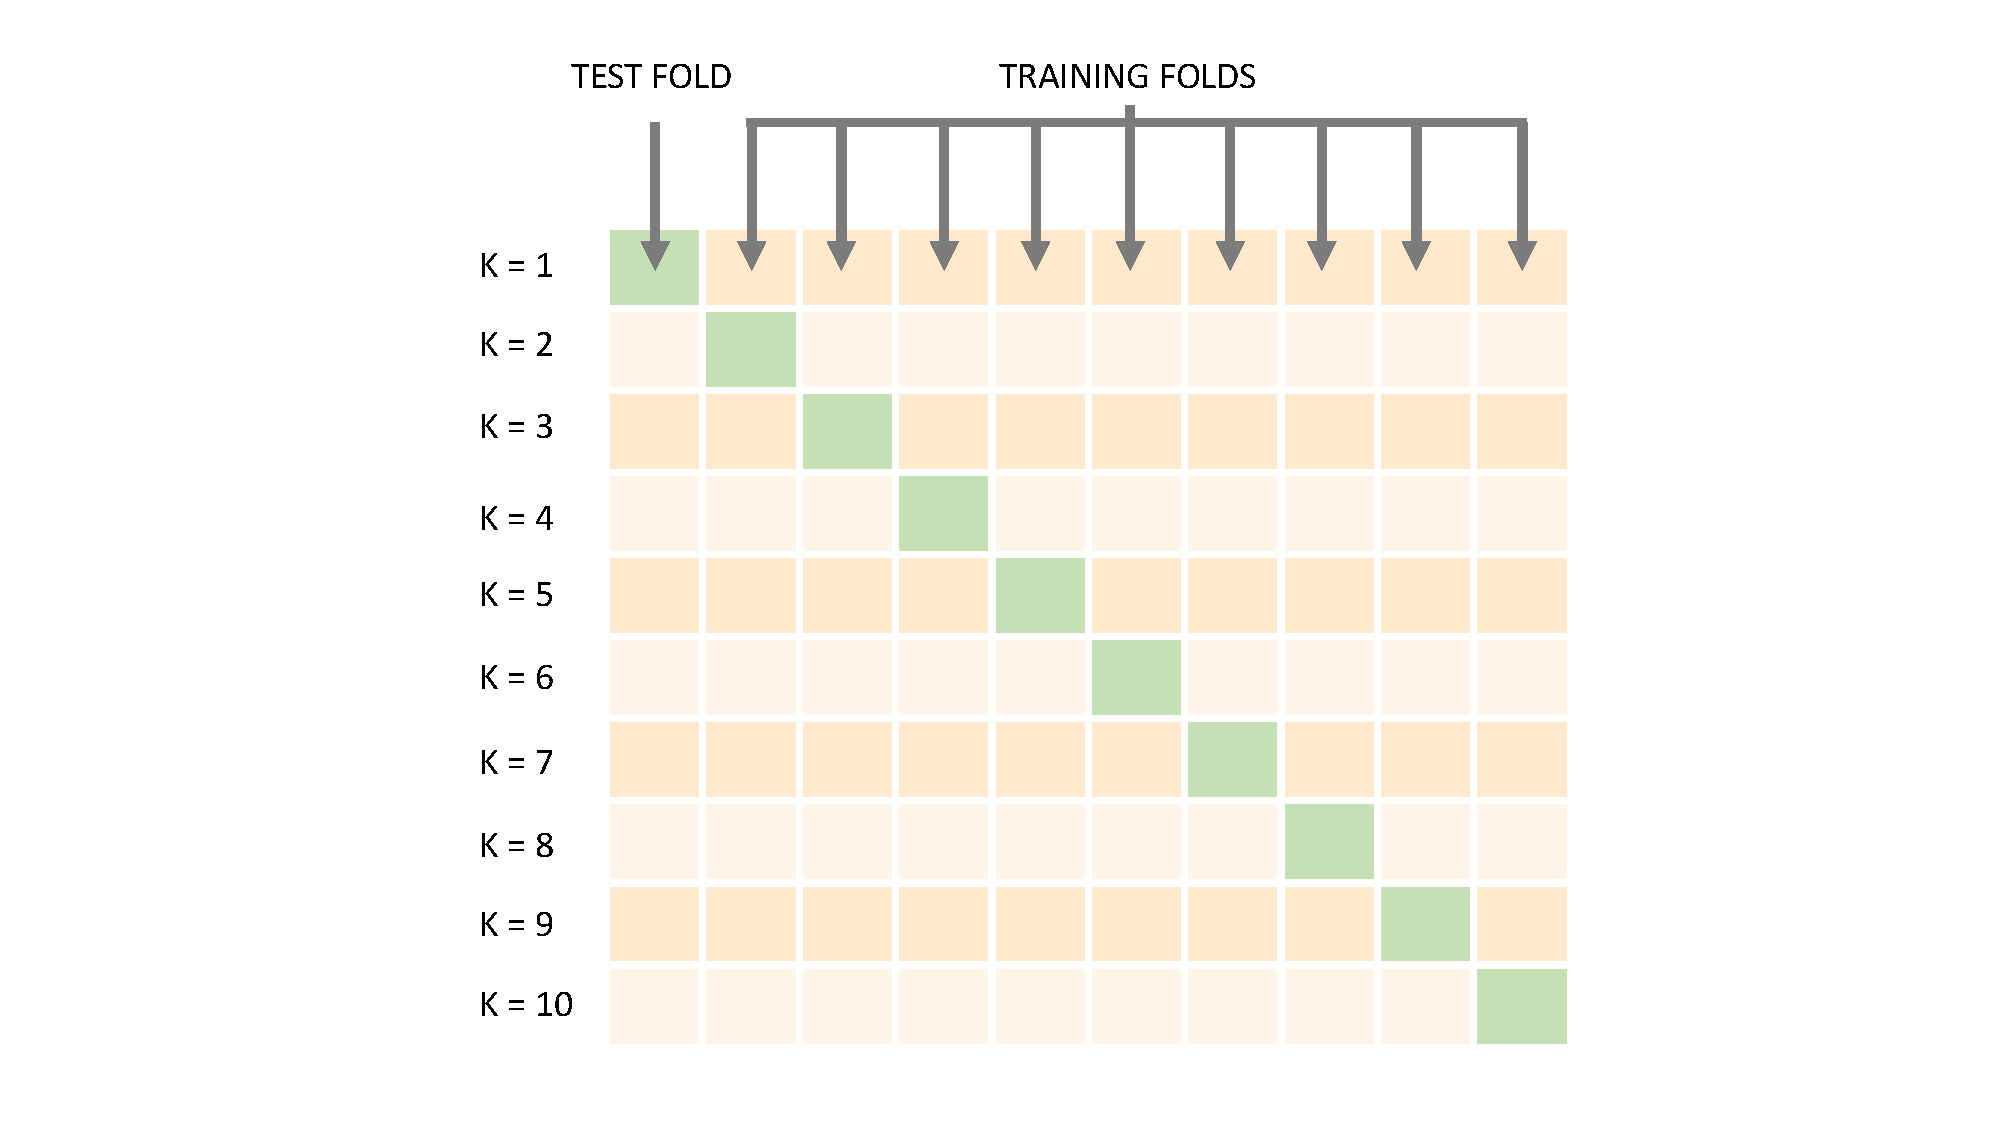
\includegraphics[width=0.8\textwidth]{"Part 3 - Learning Systems/Supervised Learning/Evaluation/Evaluation Supervised/figures/10fold-1-1.pdf"}
    \caption{10-fold cross validation scheme. The test fold is shown in green, whereas the training folds are shown in (lighter or darker) orange.}
    \label{fig:10fold}
\end{figure}

\begin{equation}
    Perf = \frac{1}{k'}\sum_{k' = 1}^{k} Perf(k')
    \label{eq:cv}
\end{equation}

\noindent where $Perf(k')$ represents any performance metric that is suitable for the problem in hands, computed on the test fold $k'$, using the classifier trained on folds $k'' \in \{1,2,\cdots,k\} \backslash k'$.




%Typically this whole procedure is repeated once for each set of classifier parameters $\Theta$ and the parameters that yield the best predictive performance are then picked to build the final classifier.


Note that $k$-fold Cross Validation does not guarantee that the best training examples will be chosen to build the classifier, however, it can be repeated as many times as necessary to reduce the chances of picking examples that do not represent well the problem.  It is also common to create the splits such that each fold preserves the same proportion of examples of each class as the proportion presented by the full data set. This process is called stratification and may help to improve the estimation of generalization.   

%In Figure \ref{fig:10fold}, as previously mentioned, 10 classifiers will be generated and evaluated on each respective test fold (green cell). In the end, the performance result is given by: 



\subsection{Leave-one-out cross-validation (LOOCV)}
\label{sec:loocv}

Leave-one-out Cross Validation (LOOCV) can be defined as a particular case of the $k$-fold Cross Validation (Section \ref{sec:cv}) where the value of $k$ is set to $n$, i.e., the total number of available labeled examples. For large datasets, using the LOOCV procedure means to create a large number of classifiers, which may be very time consuming. For small datasets, this procedure may have a feasible computational cost while enabling the models to be trained on larger training sets than when $k<n$. 

Table \ref{tab:dsloocv} shows an example of dataset containing 12 different tonalities of the colors red, green and blue. Considering this data, creating a classifier that properly generalizes this problem may be a challenging task and the $k$-fold cross validation using typical values for the $k$ may be unsuitable. Conversely, for this problem, the LOOCV will build twelve classifiers ($f$) such that each of these will be trained using 11 training examples and will be tested on the remaining one. The estimate of the generalization can then be calculated based on Eq. \ref{eq:cv} with $k=12$. 


%As for the $k$-fold Cross Validation, the LOOCV procedure is aimed to help us in finding a classifier with its specific parameters $f$ that 


\begin{table}[]
    \centering
\caption{Dataset containing different tonalities for the RGB color pattern.}
\begin{tabular}{ |p{1cm}|p{1cm}|p{1cm}|p{2cm}| } 
\hline
R & G & B & Class \\
\hline
134 & 10 & 20 & Red \\
\hline
210 & 31 & 5 & Red \\
\hline
198 & 15 & 2 & Red \\
\hline
189 & 8 & 21 & Red \\
\hline
11 & 214 & 3 & Green \\
\hline
7 & 193 & 20 & Green \\
\hline
20 & 207 & 4 & Green \\
\hline
13 & 221 & 20 & Green \\
\hline
3 & 17 & 179 & Blue \\
\hline
21 & 10 & 200 & Blue \\
\hline
12 & 18 & 215 & Blue \\
\hline
15 & 4 & 196 & Blue \\
 \hline
\end{tabular}
\label{tab:dsloocv}
\end{table}


\subsection{Repeated Hold-out Validation}
\label{sec:holdout}

The Hold-out Validation procedure simply consists in randomly selecting a given number of examples for training and using the remaining ones for testing. The training examples are used to train a predictive model $f$, whereas the test examples are used to estimate its generalization capability. However, unless the dataset is very large, using a single split of the data into training and test sets would mean that the estimate of the generalization is likely biased. By chance, the split may have been a ``lucky" one that results in a good value for the generalization estimate, when in reality the performance on other unseen examples would not be so good. Conversely, the split may have been an ``unlucky" one that results in a poor value for the generalization estimate, when in reality the performance on other unseen examples would not be so poor. 

In an attempt to overcome this issue, the Hold-out Validation procedure is typically repeated multiple times with different random splits of the data into training and test sets. The estimate of the generalization of a model trained on the full dataset is then set as the average of the test performances obtained on all repetitions. A disadvantage of this procedure compared to $k-$fold Cross Validation is that it does not ensure that every example is used for testing once. Some examples may be used multiple times for testing, whereas others may not be used at all. This could potentially lead to a more biased estimate of generalization when the dataset is not very large.

% separating the set of labeled examples in three different sets: training, validation and test datasets. The main intuition behind this procedure is that the validation dataset can help to provide a direction on whether the classifier is still learning/generalizing or not (during the training phase). 

% To illustrate this procedure, lets assume that the learning procedure of a given classifier $f$ iteratively learns from the training dataset (i.e., it passes multiple times over the training dataset). If the training dataset is presented to $f$ for only one training iteration, the classifier may not have been able to properly learn it. On the other hand, if a large number of training iterations have been performed, $f$ may overfit the data. Since the validation dataset is not used for training purposes, it can be used for assessing the learning performance of $f$ while the training phase is still in progress. 


% Table \ref{tab:holdout} shows a hypothetical scenario where a classifier learns for 10 iterations. As the training data is repeatedly presented to the classifier, it keeps learning this data and consequently, learning the validation dataset as well (since the training and validation data are produced by the same underlying generator process). We can see that at iteration 7 the validation error reach its minimum value before starting increasing again. Since the training error keeps decreasing after iteration 7, we can then conclude that the classifier is overfitting the training data and starting to worsen its generalization performance. 


% \begin{table}[]
%     \centering
% \caption{Hypothetical predictive performances for a classifier that learns based on multiple passes (iterations) over the training dataset.}
% \begin{tabular}{ |p{1.5cm}|p{1.5cm}|p{1.5cm}|p{1.5cm}| } 
% \hline
% Iteration & Training Error & Validation Error & Test Error \\
% \hline
% 1 & 43\% & 51\% & 48\% \\
% \hline
% 2 & 38\% & 46\% & 40\% \\
% \hline
% 3 & 32\% & 37\% & 41\% \\
% \hline
% 4 & 25\% & 28\% & 32\% \\
% \hline
% 5 & 19\% & 25\% & 29\% \\
% \hline
% 6 & 12\% & 14\% & 18\% \\
% \hline
% 7 & 6\% & 12\% & 16\% \\
% \hline
% 8 & 3\% & 20\% & 23\% \\
% \hline
% 9 & 2\% & 25\% & 26\% \\
% \hline
% 10 & 2\% & 30\% & 31\% \\
% \hline
% \end{tabular}
% \label{tab:holdout}
% \end{table}

% Notice that the hypothetical scenario of Table \ref{tab:holdout} may not happen exactly as it is in practice, the training and validation errors may suffer variations that increase or decrease their values while the classifier is still improving its performance generalization. Therefore, small variations in the validation error may be disregarded such that the training process stops only when the classifier start to consistently worsening its validation performance. Once the classifier is built based on the training and validation data, its generalization performance is then assessed based on the test dataset. 

% Typically, the proportions of 50\%, 25\% and 25\% of the data are used for the training, validating and testing, respectively. In addition, the data separation process must be repeated many times (lets say 30 times if possible) in order to minimize the chances of training the classifier on examples that badly represent the problem.

% As aforementioned, the main intuition behind this procedure is that the validation dataset can help to provide a direction on whether the classifier is still learning/generalizing or not. However, the holdout validation process can be applied to any classifier (i.e., not only to those ones that learn based on multiple iterations). Additionally, this procedure can be used to choose a classifier based on the validation performance and only compute the test performance for the chosen classifier. This prevents the practitioner to be tempted to pick the classifier based on the test performance, what would be methodologically wrong.


%Evaluation Procedures (George)



%1.      When introducing the evaluation procedures, explain about why we need to evaluate the models based on a dataset that is different from the training set

%2.      Talk about hyperparameter tuning --> WE CAN CANCEL THIS PART -- IT WILL BE EASIER TO TALK JUST ABOUT EVALUATING THE GENERALIZATION RATHER THAN HYPERPARAMETER TUNING. SOME COMMENTS ON HYPERPARAMETER TUNING ARE NOW IN THE SUMMARY AND DISCUSSION

%3.      Cross-validation

%4.      Leave-one-out cross-validation

%5.      Hold-out, including repeated holdout (when we repeat the procedure a number of times with different splits)




\section{Summary and Discussion}

This chapter presented evaluation procedures that can be used to evaluate the generalization ability of a predictive model $f$ learned by a given machine learning algorithm with a fixed and pre-defined set of hyperparameter values (when applicable) \footnote{Hyperparameters are parameters that have to be set before running the learning algorithm. For example, the learning rate used by backpropagation for multilayer perceptrons is a hyperparameter.}. Several different performance metrics that can be used with these evaluation procedures have also been presented, where each metric captures and/or focuses on different performance aspects. Several other performance metrics exist. As future reading, you may wish to learn about the Area Under the Receiver Operating Characteristic Curve (AUC) \cite{AUC}.

The evaluation procedures presented in this chapter are for estimating generalization. One may think of using the average test performance metrics reported by these procedures for model selection, i.e., to choose among different models created by different machine learning algorithms and/or hyperparameter values. This is possible. However, it is important to note that once the average performance metric values computed based on certain test data are used to select a model, they do not work as measures of the generalization capability of this model on unseen data anymore. This is because the model was chosen so as to optimize the value of predictive performance computed on the given test data, i.e., we chose the model (among a set of models) that does best on those test data. Therefore, such average test performance can become biased towards this chosen model  \cite{CawleyTalbot2010}. Another separate test set that was used neither for training nor for model selection would thus be necessary to further evaluate the generalization capabilities of the selected model.

\section{Exercises}

\begin{enumerate}
    \item Consider the following data set:

    \[ \mathcal{E} = \{([1,2,3], \text{positive}), ([1,1,1], \text{negative}), ([3,3,3], \text{positive})\}.\] 

    Consider also a classifier function $f$ that gives the following predictions to these examples:

    \[\{\text{negative}, \text{positive}, \text{positive}\}.\]

    Calculate all the performance metrics presented in Section \ref{sec:eval-metrics-classification} of this chapter. Reflect about the differences in the results obtained when using different metrics.

    \item Consider the following data set:

    \[ \mathcal{E} = \{([1,2,3], 1), ([1,1,1], 0.1), ([3,3,3], 7)\}.\] 

     Consider also a classifier function $f$ that gives the following predictions to these examples:

    \[\{2, 4.1, 8\}.\]

    Calculate all the performance metrics presented in Section \ref{sec:eval-metrics-regression} of this chapter. Reflect about the differences in the results obtained when using different metrics.

    \item Given the widely known dataset Iris, a $k$NN classifier with $k = 3$, and the accuracy evaluation metric, perform: (i) 10-fold cross validation, (ii) Leave-one-out cross validation and (iii) repeated hold-out validation with 30 repetitions. Analyze the results for each procedure in terms of predictive performance and training time. You may use WEKA as a machine learning tool: \url{https://www.cs.waikato.ac.nz/ml/weka/}.

\end{enumerate}

\section{Answers}

\begin{enumerate}
\item The performance values are as follows:
     \[\text{Accuracy} = \frac{1}{1+1+0+1} \approx 0.33\]
     \[\text{Classification Error} \approx 1 - 0.33 = 0.67\]
     \[\text{Precision} = \frac{1}{1+1} = 0.5\]
     \[TPR = \frac{1}{1+1} = 0.5\]
     \[FNR = \frac{1}{1+1} = 0.5\]
     \[TNR = \frac{0}{0+1} = 0\]
     \[FPR = \frac{1}{0+1} = 1\]
     \[\text{F1-Score} = 2 \cdot \frac{0.5 \cdot 0.5}{0.5 + 0.5} = 0.5\]
     \[\text{G-Mean} = \sqrt{0.5 \cdot 0} = 0\]

     Note that there are twice more positive than negative examples in $\mathcal{E}$, i.e., there is class imbalance. As most examples were misclassified, the accuracy and classification errors are poor. However, we can see that the performance on the negative class (TNR) is much worse than that on the positive class (TPR). In particular, no example of the negative class was correctly classified, leading to very low TNR. Correspondingly, the FPR was also very high. The performance on the positive class (TPR) was also poor, but not so poor (TPR = 0.5, FNR = 0.5). As the performance on the negative class was so poor, this had a dramatic impact on the value of the G-Mean (G-Mean = 0), though the impact on the F1-Score was not so large.

\item The performance values are as follows:
    \[MAE = \frac{1}{3} [|1-2| + |0.1 - 4.1| + |7-8|] = 2\]
    \[MSE = \frac{1}{3} [(1-2)^2 + (0.1-4.1)^2 + (7-8)^2] = 6\]
    \[RMSE = \sqrt{6} \approx 2.45\]
    \[MAPE = \frac{1}{3} \left[ \left| \frac{1-2}{1} \right| + \left| \frac{0.1-4.1}{0.1} \right| + \left| \frac{7-8}{7} \right|\right] = 14\]
    \[RAE = \frac{|1-2| + |0.1-4.1| + |7-8|}{|1-2.7| + |0.1 - 2.7| + |7 - 2.7|} \approx 0.70 \]
    \[RRSE = \sqrt{\frac{(1-2)^2 + (0.1-4.1)^2 + (7-8)^2}{(1-2.7)^2 + (0.1 - 2.7)^2 + (7 - 2.7)^2}} \approx 0.79\]

    Note how the large error on the second example was magnified by the RMSE and RRSE compared to the MAE and RAE metrics. Note also how the relative error on the first example ($|(1-2)/1| = 1$) was much larger than the relative error on the third example ($|(7-8)/7| = 0.14$) when calculating MAPE, despite the absolute errors (differences between the actual and predicted values) being the same for these two examples. 
\end{enumerate}


\bibliographystyle{unsrt}
\bibliography{bibliography}
